\section{Parser Combinators for Path Querying}
\label{sec:combinators}

Parser combinators is a way to specify both a language syntax and a parser for it in terms of higher-order functions. 
Parser in this framework is a function which consumes a prefix of an input and returns either a parsing result or an error if the input is erroneous. 
Parser combinators compose parsers to form more complex parsers. 
A parser combinators library usually provides a set of a basic parser combinators, such as a combinator of the sequential application of the choice, but there can also be user-defined combinators.
Most parser combinators libraries, including the Meerkat library, can only process the linear input---strings or some kind of streams.
We modify the Meerkat library to work on the graph input.

%Parser combinators provide a way to specify a language syntax in terms of functions and operations on them. 
%A parser in this framework is usually a function which consumes a prefix of an input and returns either a parsing result or an error if the input is erroneous. 
%Parsers can be composed by using a set of parser combinators to form more complex parsers. 
%A parser combinators library provides with a set of basic combinators (such as sequential application or choice), and there can also be user-defined combinators. 
%Most parser combinators libraries, including the Meerkat library, can only process the linear input --- strings or some kind of streams. 
%We extend the Meerkat library to work on the graph input.

The following ideas are at the core of the modification.
%Extension is based on some common ideas.


\begin{itemize}
\item The intersection of a context-free and a regular language is context-free. There are several constructive proofs of this fact.
The proposed solution is a yet another constructive proof with the SPPF as a user-friendly representation of the context-free grammar for the intersection.
\item Linear input can be regarded as a linear directed graph with symbols of the input labeling the edges.
\item A conventional parser moves a pointer in the input from the position $i$ to the position $i+1$ and creates a new state when token between $i$-th and $i+1$-th positions matches what is required in the grammar.
In case of graph processing, there are possibly multiple ways to move from the current vertex $i$ and it is possible to produce multiple new states.
Generalized parsing is designed to optimally handle the production of multiple new states thus it is suitable to handle graph processing.
\item Matching a token in the input can be viewed as a predicate, for example $p_c (x) = x == c$. 
We can generalize this observation allowing matching of an edge label of an arbitrary type with a predicate of some sort.
\item If vertices of the graph contain any data of interest, we can treat them in the similar fashion as the edges. We can also convert the input graph transforming vertices into edges and then querying the transformed graph.
\end{itemize}


%\begin{itemize}
%\item Intersection of context-free language and regular one is a context-free language and there are different constructive proves of this fact.
%Proposed solution is a yet another constructive prove and SPPF is a just user-friendly representation of result context-free grammar.
%\item Linear input is a simple case of graph: positions are vertices and tokens are edges labels.
%Each edge is going from position (vertex) $i$ to position (vertex) $i+1$.
%\item Parser can move pointer in input from position $i$ to position $i+1$ and create new state when token between $i$ to position $i+1$ matches with required in grammar.
%In case of graph processing there are more then one ways to go from current vertex $i$ and it is possible to get more then one new state.
%Generalized parsing is designed to optimally handle steps which produce multiple new states and can handle help to handle this situation.
%\item We can treat the fact that token in input matches with required token from grammar as a predicate.
%This observation may be generalized: we can pass through  edge if its label satisfies some predicate.
%This way we can flexibly handle labels of arbitrary types.
%\item Vertex may be converted to edge: all incoming edges are convert to oncoming into source of new edge, all outgoing are convert to outgoing from target of new edge.
%This way we can handle vertex and edge labelled graphs as edge labelled.
%\end{itemize}

\subsection{Library Structure}

Querying process in our library consists of two subprocesses listed below.
\begin{itemize}
\item Applying a query to the graph and representation it as SPPF
\item Applying semantic actions to SPPF which will allow us to retrieve all information we need from our SPPF. 
The specification we need to retrieve from SPPF also described in a terms of combinators using mapping combinators \lstinline{^} and \lstinline{&}.
In details semantic action execution is described in section~\label{sec:semanticActions} .
\end{itemize}

There are two main types of queries.
\begin{itemize}
\item Graph's edge and vertex is two main building blocks of queries. 
It is represented as a \lstinline{Edge[N]} and \lstinline{Vertex[L]} type where \lstinline{N} and \lstinline{L} is a type parameters of edge and vertex type, respectively. 
In a terms of CF-grammar edges and vertices are terminals.
There are two combinators \lstinline{E[N]} and \lstinline{V[L]} for working with basic primitives described in section \ref{sec:combinators}.
\item A complete query has a \lstinline{Query[L, N]} type.
Query is a nonterminal in a terms of CF-grammars.
For transforming an arbitrary query to a Query we have a \lstinline{syn} macro which also gives it the same name as corresponding value.
Later this naming will be used in SPPF.
\end{itemize}

\subsection{The Set of Combinators}
\label{sec:combinators}

First we introduce a small example graph which represent a map and presented in fig.~\ref{fig:graph}.
Here we have some cities which can have road between them and this relation is shown in graph as an edge with label $road\_to$.
Each city labeled with name and with a country it belongs to.

And let we try to extract some information from this map.

% \begin{figure}[h]
% 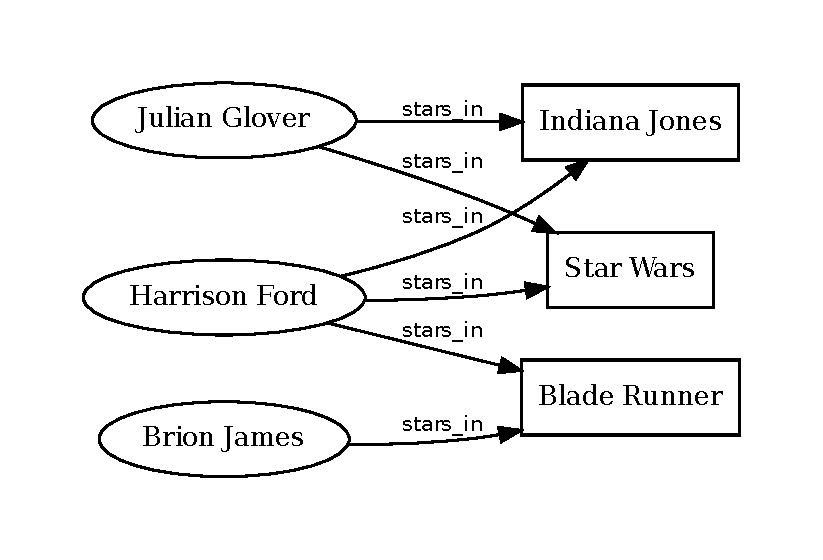
\includegraphics[width=0.45\textwidth]{graph}
% \caption{Example Input Graph of Roads}
% \label{fig:graph}
% \end{figure}

\begin{figure}[h]
\resizebox {0.45\textwidth} {!}
{
\begin{tikzpicture}[shorten >=1pt,node distance=2cm,on grid,auto] 
   \node[state] (a) [fill={rgb:black,1;white,2}]  {$a(X)$}; 
   \node[state] (b) [right=of a] {$b (Y)$}; 
   \node[state] (c) [right=of b] {$c (X)$}; 
   \node[state] (d) [left=of a] {$d (X)$};
   \node[state] (e) [left=of d] {$e (Y)$};
    \path[->] 
    (a) edge [bend left, above] node [above] {$road\_to$} (c)          
    (b) edge  node {$road\_to$} (a)
    (c) edge  node {$road\_to$} (b)
    (a) edge  node {$road\_to$} (d)
    (d) edge  node {$road\_to$} (e);
\end{tikzpicture}
}
\caption{Example Input Graph of Roads. Vertex labels in a form of "city-name (country-name)"}
\label{fig:graph}
\end{figure}

First of all, for creating queries we need to work with edges and vertices.
There are two main functions for that:
\begin{itemize}
    \item \lstinline{V[L](predicate: L => Boolean)} combinator for working with vertices. Accepts a predicate and parses only vertices which satisfies that predicate
    \item \lstinline{E[N](predicate: N => Boolean)} combinator for working with edges. Accepts a predicate and parses only edges which satisfies that predicate  
\end{itemize}

\begin{figure}[h]
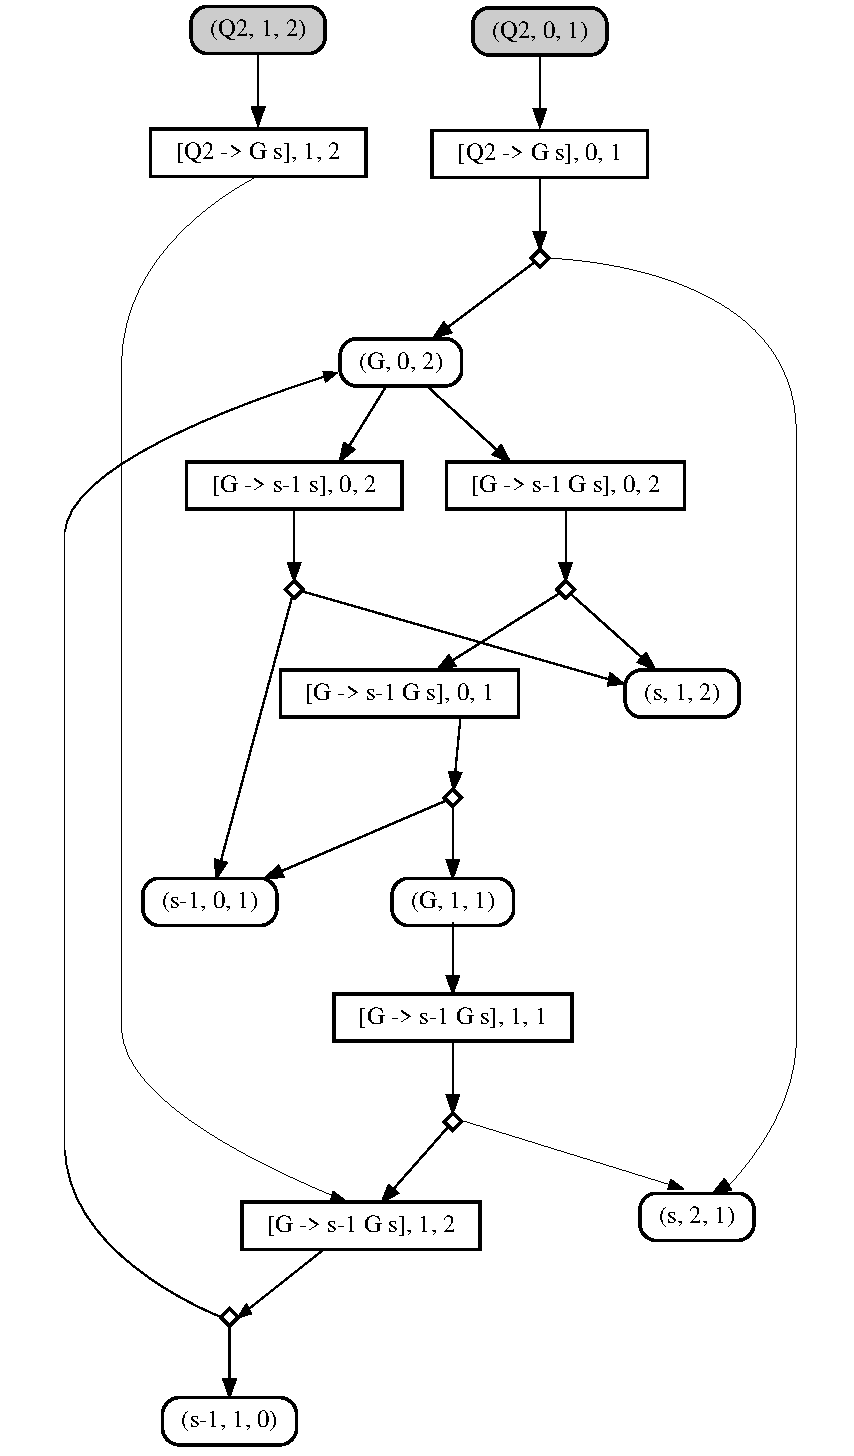
\includegraphics[width=0.49\textwidth]{sppf}
\caption{SPPF: result of applying cities query to the graph~\ref{fig:graph}}
\label{fig:sppf}
\end{figure}




Suppose that we would like to select cities from our graph which belongs to some country. 
For that we use function \lstinline{V}: \lstinline{V[L]((e: Entity) => e.country = "County Name")}.
Here \lstinline{Entity} is a property container for graph entities: edges and vertices. All properties usings (like \lstinline{(e: Entity).country}) are converted to the corresponding graph entity properties using Scala's \lstinline{Dynamic} trait.
Also, for the sake of simplicity, we will not explicitly specify \lstinline{Entity} type for predicates. 
Now let us build a query which gets all roads from city in country $X$ to the city in country $Y$. 
For that we can use a sequentialital combinator \lstinline{~}. 
It allows to create queries which sequentialy applies two queries one after another. 
When we have subquery for retrieving a vertex with specific city, let's call it \lstinline{city(name: String)} and a subquery \lstinline{roadTo} for retrieving road edges. 
Let us finally build a query \lstinline{city("X") ~ roadTo ~ city("Y")} which will give us requested set of paths from our graph.
The full query with subqueries is shown on fig. \ref{fig:simpleQuery}.

\begin{figure}[h]
\begin{lstlisting}
def city(country: String) =
  V(e.country == country)
val roadTo = E(_.value() == "road_to")
val ourPath = 
  city("X") ~ roadTo ~ city("Y")
\end{lstlisting}
\caption{Path query}
\label{fig:simpleQuery}
\end{figure}



Now we would like to get all pair of cities which have a road between them. 
So we need to transform our query to use semantic actions which is described in \ref{sec:semanticActions} section. 
Now let us specify what we want from every our query. 
From the \lstinline{city} query we want only city name, so we need to map a result of basic vertex combinator. 
For that case we have a \lstinline{^} combinator we can write \lstinline{def city(name: String) = syn(V(e.value() == name) ^ (_.value))} to achive that. 
In \lstinline{ourPath} query we need first and second cities to be represented as a pair. 
For that we have a \lstinline{&} combinator which will map our sequence to a pair of strings.
The final representation is shown on \ref{fig:simpleQueryV2}. 
Now when we execute that query we will get a list which consists of all pairs of city's names which have a road between.

\begin{figure}[h]
\begin{lstlisting}
def city(country: String) =
  syn(V(e.country() == country) ^ (_.name))
val roadTo = E(_.value() == "road_to")
val ourPath = 
  syn(city("X") ~ roadTo ~ city("Y") &
    { case c0 ~ c1 => (c1, c2) }
\end{lstlisting}
\caption{Path query}
\label{fig:simpleQueryV2}
\end{figure}


The whole set of basic combinators our library provides are presented in table~\ref{table:combinators}. 
It consists of two kind of combinators. The first kind creates new parsers from existing ones, meanwhile the second one allows mapping parsers result.
Parsers for matching strings are implicitly generated whenever a string is used within a query. 



\begin{table}[h]
\centering
\begin{tabular}{l@{}|l}
\multicolumn{1}{c|}{Combinator} & \multicolumn{1}{|c}{Description} \\ \hline
{\lstinline!a ~ b!} & sequential parsing: {\lstinline!a!} then {\lstinline!b!}   \\
{\lstinline!a | b!} & choice: {\lstinline!a!} or {\lstinline!b!}         \\
{\lstinline!a ?!}   & optional parsing: {\lstinline!a!} or nothing   \\
{\lstinline!a *!}   & repetition of zero or more {\lstinline!a!} \\
{\lstinline!a +!}   & repetition of at least one {\lstinline!a!} \\
{\lstinline!a ^ f!} & apply {\lstinline!f!} function to {\lstinline!a!} if  {\lstinline!a!} is a token \\
{\lstinline!a ^^!}  & capture output of {\lstinline!a!} if {\lstinline!a!} is a token    \\
{\lstinline!a & f!} & apply {\lstinline!f!} function to {\lstinline!a!} if  {\lstinline!a!} is a parser \\
{\lstinline!a &&!}  & capture output of {\lstinline!a!} if {\lstinline!a!} is a parser    \\
\hline
\end{tabular}
\caption{Meerkat combinators}
\label{table:combinators}
\end{table}


\subsection{Generic interface for input}
Combinators is a generic way to describe a query and when we have a query we want to execute that query on some graph considering it as an input for our query.
The cool thing is that query execution mechanism may be fully separated from graph representation.
We need only to have access to two very low-level functions, one for working with edges and one for vertices. 
The first one would allow to get all edges outcoming from current vertex and also satisfies given predicate. 
The second one will allow to check if current vertex satisfies given predicate.
That interface is presented on fig~.\ref{fig:input}.
It has two type parameters: \lstinline{L} for edge labels and \lstinline{N} for nodes.
We have implementation of that input for the next data sources: 

\begin{itemize}
    \item Neo4jInput --- input source for working with graph database Neo4J;
    \item GraphxInput --- input source for working with graph presented in memory using GraphX library;
    \item LinearInput --- input source for working with linear input data like strings.
\end{itemize}

\begin{figure}[h]
\begin{lstlisting}
trait Input[+L, +N] {
  def filterEdges(nodeId: Int, 
      predicate: L => Boolean): Seq[(L, Int)]
  def checkNode(nodeId: Int, 
      predicate: N => Boolean): Option[N]
}

\end{lstlisting}
\caption{Generalized input interface}
\label{fig:input}
\end{figure}

As far as required functions is very simple, we hope that this interface can be implemented for arbitrary storage of graph-structured data.
Note, that currently we use \lstinline{Int} as unique identifier for nodes (the \lstinline{nodeId} parameter).
It may be a technical restriction by the next two reason.
\begin{itemize}
\item It is impossible to use our library for correct processing of graph with more then \lstinline{MAX_INT} nodes). 
\item It is necessary to provide such identifiers. Many systems use unique identifiers by default, but in some cases it may be necessary to implement required functionality manually.
\end{itemize}



\subsection{Semantic Actions}
\label{sec:semanticActions}
Each path query produces a parse result stored in SPPF.
This representation is very rich but hard to use and understand.
That is why our library provides a mechanism which allows you to extract and process any useful data stored in parse result.
This mechanism is called semantic actions.
In general, they give you an opportunity to apply any function to parsed token or sequence.
Now, let's understand how actions can be used in queries and how they are implemented in our library.

There are two main semantic action binders \lstinline{^} and \lstinline{&}.
First of them is used when we need to perform some action on primitive tokens such as vertices or edges.
\begin{lstlisting}
// Defined in Terminal[+L] (edge) parser
def ^[U](f: L => U) = 
  new SymbolWithAction[L, Nothing, U] {...
  
// Defined in Vertex[+N] parser
def ^[U](f: N => U) = 
  new SymbolWithAction[Nothing, N, U] {...
\end{lstlisting}

Second is used when we need to process a result of combination of parsers.
\begin{lstlisting}
// Defined in Symbol[+L, +N, +V] parser
def &[U](f: V => U) = 
  new SymbolWithAction[L, N, U] {...
\end{lstlisting}

But actually, they both have the same behaviour, they produce a new parser that has the same parsing possibilities as an original parser but also have a binded function.
Then, every SPPF node that will be produced by parser with binded function will have a reference to this function too.

So, these operations in composition with other combinators provides an instrument for data processing on which most queries are based. 
For example, \lstinline{^} can extract some data from tokens and \lstinline{&} applied to sequence of tokens can collect and process data returned by terminal parsers.

The main idea of execution of semantic actions remained the same as in the original Meerkat library excepting one aspect.
For each node we still just execute all actions of its children, collect results and pass them as argument to current function.
But what should executor do if SPPF has ambiguous nodes? 
Previous implementation just throws an exception in that case and it is reasonable because original library is written for linear parsing and most grammars allows disambiguation in that case.

However, even unambiguous grammar can produce ambiguous derivations during parsing of graphs.
That's why we provide a feature that makes it possible to extract ``all'' trees stored in SPPF.
The number of path deriving from given grammar can be infinite, for example, when graph has cycles.
This reason we can provide only a lazy stream of trees that allows to take as much of them as you need.
Our solution is based on breadth first search that yields an unambiguous SPPF corresponding to some derivation immediately after it was found.

Composition of trees extraction and semantic action execution gives us a function that we called \lstinline{executeQuery}.
It parses graph from all positions producing a list of SPPF roots, then it extracts all derivations from all roots, executes semantic actions and returns a stream of results.